\documentclass{standalone}
\usepackage{tikz}
\usetikzlibrary{patterns, positioning}
\usepackage[sfdefault]{ClearSans} %% option 'sfdefault' activates Clear Sans as the default text font
\usepackage[T1]{fontenc}

\begin{document}
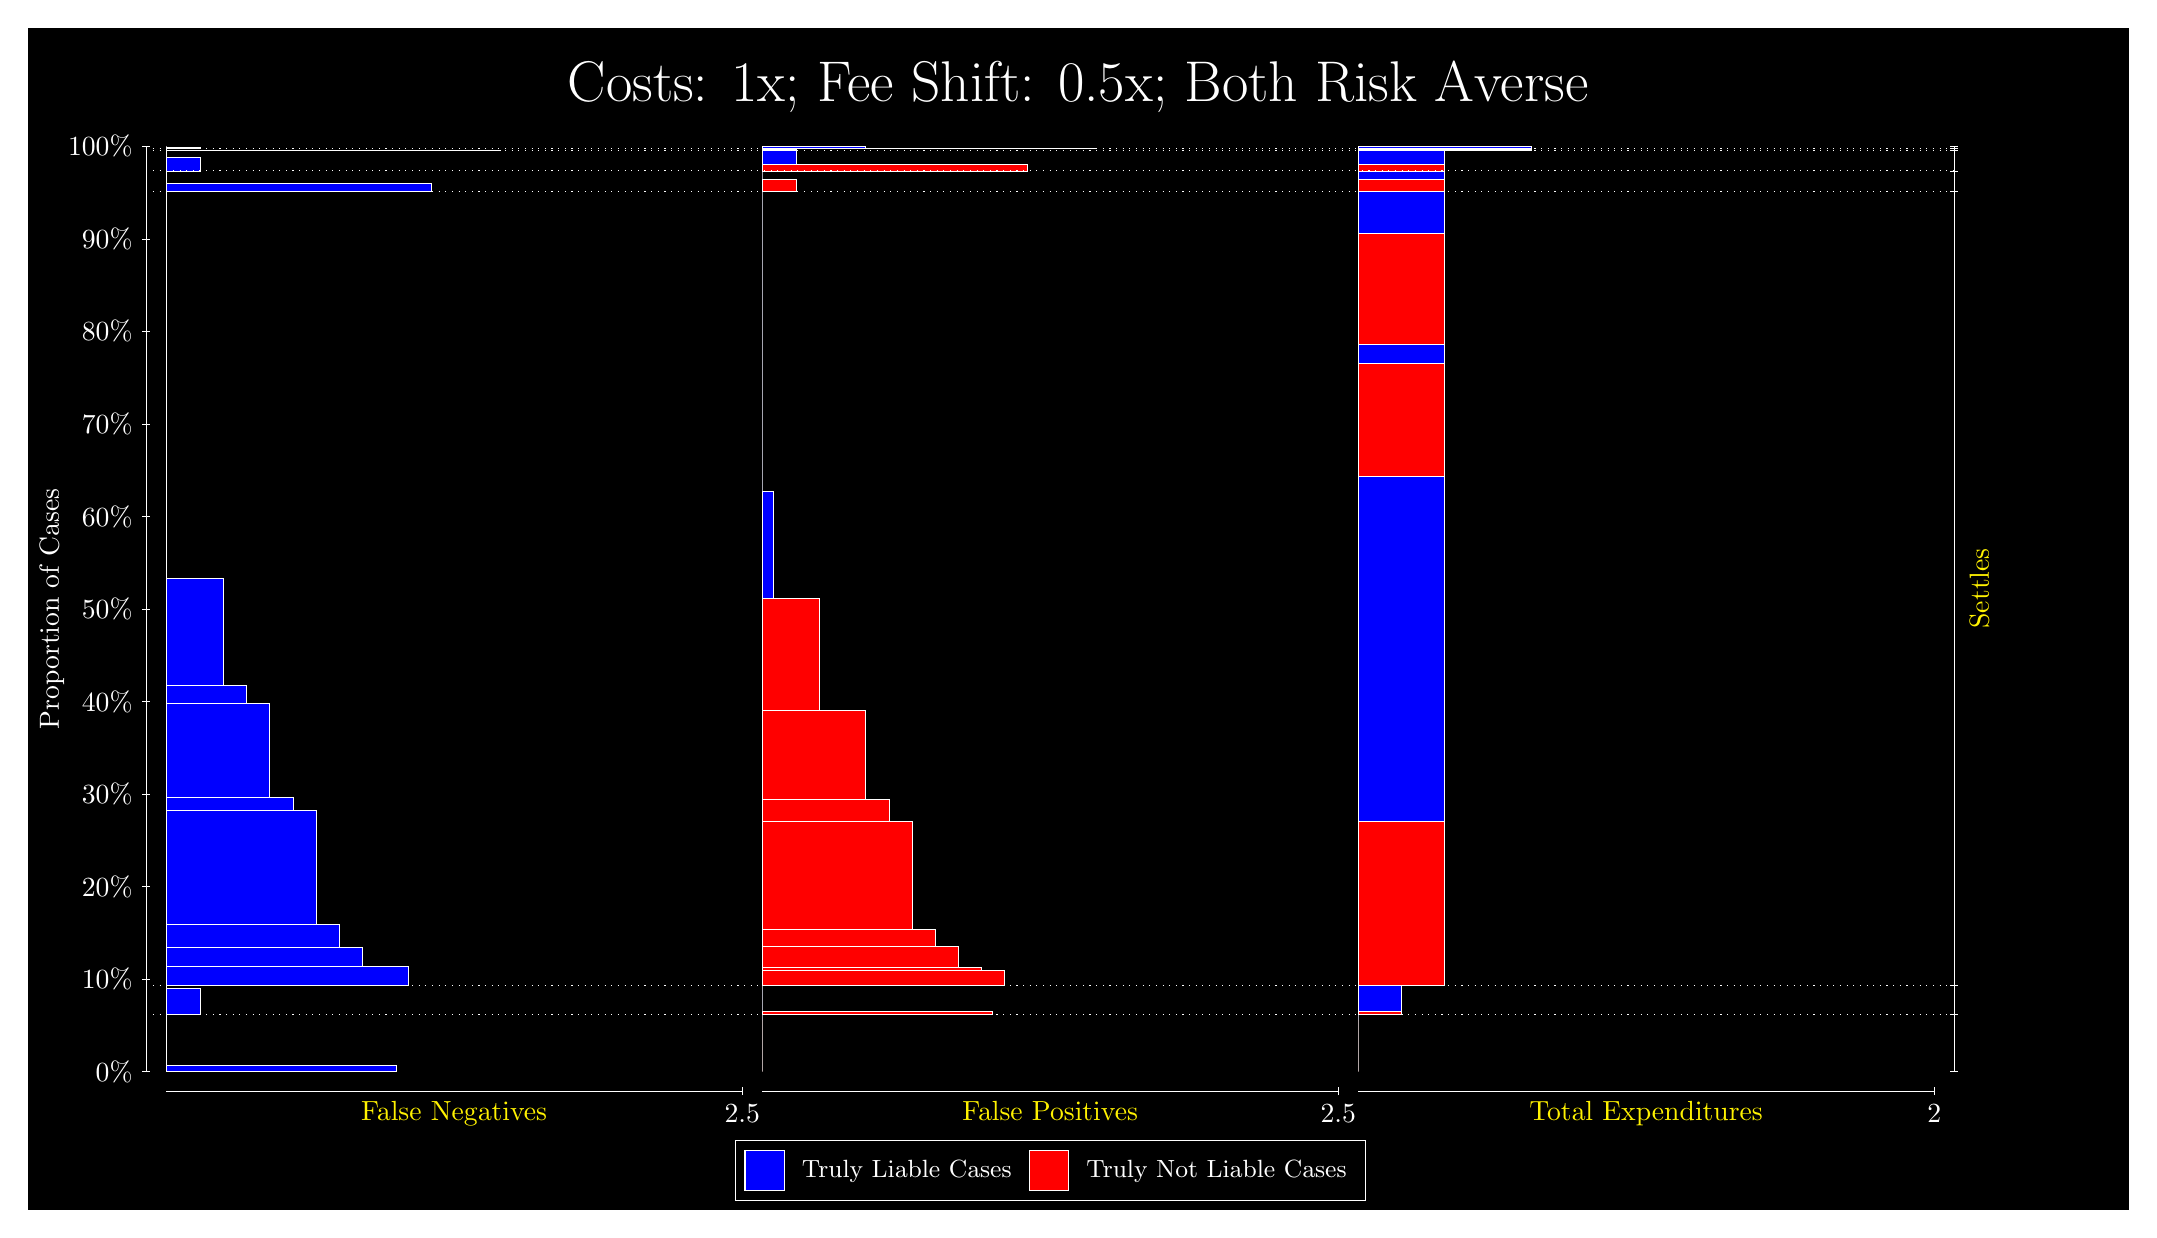
\begin{tikzpicture}
\draw[fill=black] (0,0) rectangle (26.667,15);
\draw[text=white] (0,13.5) rectangle (26.667,15) node[midway] {\huge Costs: 1x; Fee Shift: 0.5x; Both Risk Averse};
\draw[white, very thin] (1.5,1.75) -- (1.5,13.5);
\node[rotate=90, text=white, anchor=center] at (0.3, 7.625) {Proportion of Cases};
\draw[white, very thin] (1.45,1.75) -- (1.55,1.75);
\node[text=white, anchor=east] at (1.45, 1.75) {0\%};
\draw[white, very thin] (1.45,2.925) -- (1.55,2.925);
\node[text=white, anchor=east] at (1.45, 2.925) {10\%};
\draw[white, very thin] (1.45,4.1) -- (1.55,4.1);
\node[text=white, anchor=east] at (1.45, 4.1) {20\%};
\draw[white, very thin] (1.45,5.275) -- (1.55,5.275);
\node[text=white, anchor=east] at (1.45, 5.275) {30\%};
\draw[white, very thin] (1.45,6.45) -- (1.55,6.45);
\node[text=white, anchor=east] at (1.45, 6.45) {40\%};
\draw[white, very thin] (1.45,7.625) -- (1.55,7.625);
\node[text=white, anchor=east] at (1.45, 7.625) {50\%};
\draw[white, very thin] (1.45,8.8) -- (1.55,8.8);
\node[text=white, anchor=east] at (1.45, 8.8) {60\%};
\draw[white, very thin] (1.45,9.975) -- (1.55,9.975);
\node[text=white, anchor=east] at (1.45, 9.975) {70\%};
\draw[white, very thin] (1.45,11.15) -- (1.55,11.15);
\node[text=white, anchor=east] at (1.45, 11.15) {80\%};
\draw[white, very thin] (1.45,12.325) -- (1.55,12.325);
\node[text=white, anchor=east] at (1.45, 12.325) {90\%};
\draw[white, very thin] (1.45,13.5) -- (1.55,13.5);
\node[text=white, anchor=east] at (1.45, 13.5) {100\%};

\draw[white, very thin] (24.457,1.75) -- (24.457,13.5);
\draw[white, very thin] (24.407,1.75) -- (24.507,1.75);
\node[anchor=west] at (24.407, 1.75) {};
\draw[white, very thin] (24.407,2.4788) -- (24.507,2.4788);
\node[anchor=west] at (24.407, 2.4788) {};
\draw[white, very thin] (24.407,2.8431) -- (24.507,2.8431);
\node[anchor=west] at (24.407, 2.8431) {};
\draw[white, very thin] (24.407,12.93) -- (24.507,12.93);
\node[anchor=west] at (24.407, 12.93) {};
\draw[white, very thin] (24.407,13.188) -- (24.507,13.188);
\node[anchor=west] at (24.407, 13.188) {};
\draw[white, very thin] (24.407,13.445) -- (24.507,13.445);
\node[anchor=west] at (24.407, 13.445) {};
\draw[white, very thin] (24.407,13.47) -- (24.507,13.47);
\node[anchor=west] at (24.407, 13.47) {};
\draw[white, very thin] (24.407,13.5) -- (24.507,13.5);
\node[anchor=west] at (24.407, 13.5) {};

\draw[white, very thin, fill=blue] (1.75,1.75) rectangle (4.6775,1.8267);
\draw[white, very thin, fill=red] (1.75,1.8267) rectangle (1.75,2.4788);
\draw[white, very thin, fill=blue] (1.75,2.4788) rectangle (2.1891,2.8048);
\draw[white, very thin, fill=red] (1.75,2.8048) rectangle (1.75,2.8431);
\draw[white, very thin, fill=blue] (1.75,2.8431) rectangle (4.8239,3.0877);
\draw[white, very thin, fill=blue] (1.75,3.0877) rectangle (4.2384,3.3314);
\draw[white, very thin, fill=blue] (1.75,3.3314) rectangle (3.9457,3.6246);
\draw[white, very thin, fill=blue] (1.75,3.6246) rectangle (3.6529,5.0712);
\draw[white, very thin, fill=blue] (1.75,5.0712) rectangle (3.3602,5.2381);
\draw[white, very thin, fill=blue] (1.75,5.2381) rectangle (3.0674,6.4254);
\draw[white, very thin, fill=blue] (1.75,6.4254) rectangle (2.7746,6.6572);
\draw[white, very thin, fill=blue] (1.75,6.6572) rectangle (2.4819,8.0122);
\draw[white, very thin, fill=red] (1.75,8.0122) rectangle (1.75,12.93);
\draw[white, very thin, fill=blue] (1.75,12.93) rectangle (5.1167,13.031);
\draw[white, very thin, fill=red] (1.75,13.031) rectangle (1.75,13.188);
\draw[white, very thin, fill=blue] (1.75,13.188) rectangle (2.1891,13.36);
\draw[white, very thin, fill=red] (1.75,13.36) rectangle (1.75,13.445);
\draw[white, very thin, fill=blue] (1.75,13.445) rectangle (5.9949,13.454);
\draw[white, very thin, fill=red] (1.75,13.454) rectangle (1.75,13.47);
\draw[white, very thin, fill=blue] (1.75,13.47) rectangle (2.1891,13.491);
\draw[white, very thin, fill=red] (1.75,13.491) rectangle (1.75,13.5);
\draw[white, very thin, fill=red] (9.3189,1.75) rectangle (9.3189,2.4021);
\draw[white, very thin, fill=blue] (9.3189,2.4021) rectangle (9.3189,2.4788);
\draw[white, very thin, fill=red] (9.3189,2.4788) rectangle (12.246,2.5171);
\draw[white, very thin, fill=blue] (9.3189,2.5171) rectangle (9.3189,2.8431);
\draw[white, very thin, fill=red] (9.3189,2.8431) rectangle (12.393,3.0362);
\draw[white, very thin, fill=red] (9.3189,3.0362) rectangle (12.1,3.0729);
\draw[white, very thin, fill=red] (9.3189,3.0729) rectangle (11.807,3.345);
\draw[white, very thin, fill=red] (9.3189,3.345) rectangle (11.515,3.5567);
\draw[white, very thin, fill=red] (9.3189,3.5567) rectangle (11.222,4.9279);
\draw[white, very thin, fill=red] (9.3189,4.9279) rectangle (10.929,5.2104);
\draw[white, very thin, fill=red] (9.3189,5.2104) rectangle (10.636,6.3351);
\draw[white, very thin, fill=red] (9.3189,6.3351) rectangle (10.051,7.7605);
\draw[white, very thin, fill=blue] (9.3189,7.7605) rectangle (9.4652,9.1155);
\draw[white, very thin, fill=blue] (9.3189,9.1155) rectangle (9.3189,12.93);
\draw[white, very thin, fill=red] (9.3189,12.93) rectangle (9.758,13.087);
\draw[white, very thin, fill=blue] (9.3189,13.087) rectangle (9.3189,13.188);
\draw[white, very thin, fill=red] (9.3189,13.188) rectangle (12.686,13.273);
\draw[white, very thin, fill=blue] (9.3189,13.273) rectangle (9.758,13.445);
\draw[white, very thin, fill=red] (9.3189,13.445) rectangle (9.758,13.461);
\draw[white, very thin, fill=blue] (9.3189,13.461) rectangle (9.3189,13.47);
\draw[white, very thin, fill=red] (9.3189,13.47) rectangle (13.564,13.479);
\draw[white, very thin, fill=blue] (9.3189,13.479) rectangle (10.636,13.5);
\draw[white, very thin, fill=red] (16.888,1.75) rectangle (16.888,2.4021);
\draw[white, very thin, fill=blue] (16.888,2.4021) rectangle (16.888,2.4788);
\draw[white, very thin, fill=red] (16.888,2.4788) rectangle (17.437,2.5171);
\draw[white, very thin, fill=blue] (16.888,2.5171) rectangle (17.437,2.8431);
\draw[white, very thin, fill=red] (16.888,2.8431) rectangle (17.986,4.9279);
\draw[white, very thin, fill=blue] (16.888,4.9279) rectangle (17.986,9.3155);
\draw[white, very thin, fill=red] (16.888,9.3155) rectangle (17.986,10.741);
\draw[white, very thin, fill=blue] (16.888,10.741) rectangle (17.986,10.985);
\draw[white, very thin, fill=red] (16.888,10.985) rectangle (17.986,12.393);
\draw[white, very thin, fill=blue] (16.888,12.393) rectangle (17.986,12.93);
\draw[white, very thin, fill=red] (16.888,12.93) rectangle (17.986,13.087);
\draw[white, very thin, fill=blue] (16.888,13.087) rectangle (17.986,13.188);
\draw[white, very thin, fill=red] (16.888,13.188) rectangle (17.986,13.273);
\draw[white, very thin, fill=blue] (16.888,13.273) rectangle (17.986,13.445);
\draw[white, very thin, fill=red] (16.888,13.445) rectangle (19.083,13.461);
\draw[white, very thin, fill=blue] (16.888,13.461) rectangle (19.083,13.47);
\draw[white, very thin, fill=red] (16.888,13.47) rectangle (19.083,13.479);
\draw[white, very thin, fill=blue] (16.888,13.479) rectangle (19.083,13.5);
\draw[white, dotted] (1.5,2.4788) -- (24.457,2.4788);
\draw[white, dotted] (1.5,2.8431) -- (24.457,2.8431);
\draw[white, dotted] (1.5,12.93) -- (24.457,12.93);
\draw[white, dotted] (1.5,13.188) -- (24.457,13.188);
\draw[white, dotted] (1.5,13.445) -- (24.457,13.445);
\draw[white, dotted] (1.5,13.47) -- (24.457,13.47);
\draw[white, very thin] (1.75,1.5) -- (9.0689,1.5);
\node[text=yellow, anchor=north] at (5.4094, 1.5) {False Negatives};
\draw[white, very thin] (9.0689,1.45) -- (9.0689,1.55);
\node[text=white, anchor=north] at (9.0689, 1.45) {2.5};

\draw[white, very thin] (9.3189,1.5) -- (16.638,1.5);
\node[text=yellow, anchor=north] at (12.978, 1.5) {False Positives};
\draw[white, very thin] (16.638,1.45) -- (16.638,1.55);
\node[text=white, anchor=north] at (16.638, 1.45) {2.5};

\draw[white, very thin] (16.888,1.5) -- (24.207,1.5);
\node[text=yellow, anchor=north] at (20.547, 1.5) {Total Expenditures};
\draw[white, very thin] (24.207,1.45) -- (24.207,1.55);
\node[text=white, anchor=north] at (24.207, 1.45) {2};



\node[text=yellow, centered, rotate=90] at (24.777, 7.8863) {Settles};





\draw (12.978300999999998,1.5) node[draw=none] (baseCoordinate) {};
\begin{scope}[align=center]
        \matrix[scale=0.5, draw=white, below=0.5cm of baseCoordinate, nodes={draw}, column sep=0.1cm]{
            \node[rectangle, draw, minimum width=0.5cm, minimum height=0.5cm, fill=blue] {}; &
            \node[draw=none, font=\small, text=white] (B) {Truly Liable Cases}; &
            \node[rectangle, draw, minimum width=0.5cm, minimum height=0.5cm, fill=red] {}; &
            \node[draw=none, font=\small, text=white] (B) {Truly Not Liable Cases}; \\
            };
\end{scope}

\end{tikzpicture}
\end{document}